\section{Vector Fields and Differential Forms}
\label{sec:sec1}

We start by defining the tangent space of a manifold at a particular point, given the definition of tangent vector.

\begin{definition}
    The \emph{tangent space} of a manifold $M$ at $q \in M$ is defined by the set of all tangent vectors at $q$.
\end{definition}

It is possible to map the tangent space $T_q M$ at $q \in M$ to a real vector space $\mathbb{R}^n$ through a bijection.
This bijection can be used to transfer the vector space operations of $\mathbb{R}^n$ to $T_q M$, thus turning the latter into a real vector space of dimension $n$.

\begin{definition}
    We define the \emph{dimension} of a manifold $M$ as
    \begin{equation*}
        \dim M \coloneqq \dim T_q M , \quad q \in M .
    \end{equation*}
\end{definition}

If we assemble together all the tangent vectors at all points $q$ of a manifold, we obtain the tangent bundle.

\begin{definition}
    The \emph{tangent bundle} of a manifold $M$ is given by the disjoint union of all vector spaces on a manifold, thus
    \begin{equation*}
        TM \coloneqq \bigsqcup _{q \in M} T_q M .
    \end{equation*}
\end{definition}

An element of $TM$ is a pair $(q, v)$, where $q \in M$ and $v \in T_q M$.
There is a natural projection
\begin{align*}
    \pi : TM &\rightarrow M \\
    (q, v) &\mapsto q .
\end{align*}
Then the \emph{fiber} at $q \in M$ is $\pi ^{-1} (q)$.

More generally we can define a vector bundle over a manifold.

\begin{definition}
    A \emph{vector bundle} of rank $r$ is a triple $(E, \pi, M)$, where $E$ is an $r$-dimensional manifold called the \emph{total space}, $M$ is a manifold called the \emph{base space} and $\pi : E \rightarrow M$ is a continuous surjective map.
\end{definition}

We call the $r$-dimensional vector space $E_q \coloneqq \pi^{-1}(q)$ the \emph{fiber} at $q \in M$.
The tangent space is already an example of tangent bundle.

\begin{example}
    The Möbius strip is a vector bundle of rank $1$ over the circle $S^1$ (see \Cref{fig:Mobius}). Note that the product manifold $[-1, 1] \times S^1$ would be a cylinder, not the Möbius strip.
\end{example}

\begin{figure}
    \centering
    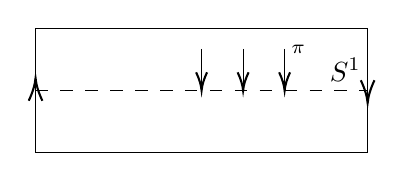
\begin{tikzpicture}[x=0.75pt,y=0.75pt,yscale=-1,xscale=1]
    %uncomment if require: \path (0,300); %set diagram left start at 0, and has height of 300
    
    %Straight Lines [id:da575614681710741] 
    \draw    (150,90) -- (310,90) ;
    %Straight Lines [id:da7355250432830472] 
    \draw    (150,150) -- (310,150) ;
    %Straight Lines [id:da425921249207598] 
    \draw  [dash pattern={on 4.5pt off 4.5pt}]  (150,120) -- (310,120) ;
    %Straight Lines [id:da15541437714065776] 
    \draw    (150,150) -- (150,90) ;
    \draw [shift={(150,114)}, rotate = 90] [color={rgb, 255:red, 0; green, 0; blue, 0 }  ][line width=0.75]    (10.93,-3.29) .. controls (6.95,-1.4) and (3.31,-0.3) .. (0,0) .. controls (3.31,0.3) and (6.95,1.4) .. (10.93,3.29)   ;
    %Straight Lines [id:da40082781733479333] 
    \draw    (310,90) -- (310,150) ;
    \draw [shift={(310,126)}, rotate = 270] [color={rgb, 255:red, 0; green, 0; blue, 0 }  ][line width=0.75]    (10.93,-3.29) .. controls (6.95,-1.4) and (3.31,-0.3) .. (0,0) .. controls (3.31,0.3) and (6.95,1.4) .. (10.93,3.29)   ;
    %Straight Lines [id:da6754846896588976] 
    \draw    (270,100) -- (270,118) ;
    \draw [shift={(270,120)}, rotate = 270] [color={rgb, 255:red, 0; green, 0; blue, 0 }  ][line width=0.75]    (8.74,-2.63) .. controls (5.56,-1.12) and (2.65,-0.24) .. (0,0) .. controls (2.65,0.24) and (5.56,1.12) .. (8.74,2.63)   ;
    %Straight Lines [id:da23038618406097078] 
    \draw    (250,100) -- (250,118) ;
    \draw [shift={(250,120)}, rotate = 270] [color={rgb, 255:red, 0; green, 0; blue, 0 }  ][line width=0.75]    (8.74,-2.63) .. controls (5.56,-1.12) and (2.65,-0.24) .. (0,0) .. controls (2.65,0.24) and (5.56,1.12) .. (8.74,2.63)   ;
    %Straight Lines [id:da41624213159172174] 
    \draw    (230,100) -- (230,118) ;
    \draw [shift={(230,120)}, rotate = 270] [color={rgb, 255:red, 0; green, 0; blue, 0 }  ][line width=0.75]    (8.74,-2.63) .. controls (5.56,-1.12) and (2.65,-0.24) .. (0,0) .. controls (2.65,0.24) and (5.56,1.12) .. (8.74,2.63)   ;
    
    % Text Node
    \draw (272,100) node [anchor=west] [inner sep=0.75pt]  [font=\scriptsize] [align=left] {$\displaystyle \pi $};
    % Text Node
    \draw (308,117) node [anchor=south east] [inner sep=0.75pt]   [align=left] {$\displaystyle S^{1}$};
    
    
\end{tikzpicture}
    \caption{Construction of the Möbius strip.}
    \label{fig:Mobius}
\end{figure}

We introduce now the definition of a section, which will be essential to define vector fields and differential $1$-forms.

\begin{definition}
    Let $(E, \pi, M)$ be a vector bundle. A \emph{section} on an open subset $U \subset M$ is a continuous map $\sigma : U \rightarrow E$ such that $\pi \circ \sigma = \text{id}_U$.
\end{definition}

We will denote the space of sections of a vector bundle $(E, \pi, M)$ by $\Gamma(E)$.

\begin{definition}
    A section $X \in \Gamma(TM)$ of the tangent bundle of a manifold $M$ is called a \emph{vector field}.
\end{definition}

A vector field is nothing else than a choice of a tangent vector at a point $q$ for all points $q \in M$.
We will denote the space of vector fields on a manifold $M$ by $\mathfrak{X}(M) \coloneqq \Gamma(TM)$.
In local coordinates ($x^i$) on $M$, we can write a vector field $X \in \mathfrak{X}(M)$ as

\begin{equation*}
    X = \sum_{i=1}^n X^i \frac{\partial}{\partial x^i}.
\end{equation*}

In particular, if $M = \mathbb{R}^n$, $X$ a smooth vector field and $f$ a smooth map, then we can define

\begin{equation*}
    X(f) = \sum_{i=1}^n X^i \frac{\partial f}{\partial x^i} .
\end{equation*}

\begin{definition}
    The \emph{cotangent bundle} $T^*M$ of a manifold $M$ is the dual of the tangent bundle $TM$.
\end{definition}

Similarly to what we did to define vector spaces, we can now introduce the concept of differential $1$-forms.

\begin{definition}
    A section $\omega \in \Gamma(T^*M)$ of the cotangent bundle of a manifold $M$ is called a \emph{differential $1$-form}.
\end{definition}

We denote by $\Omega^1(M) \coloneqq \Gamma(T^*M)$ the space of differential $1$-forms.

We now introduce the notion of tensor bundle in order to generalize vector fields and differential $1$-forms to multivector fields and differential $s$-forms, respectively.
We will then define the de Rham differential on $s$-forms, the Lie derivative and the contraction of a vector field with an $s$-form.

\begin{definition}
    Assume $(E, \pi, M)$ is a vector bundle over $M$.
    We define the \emph{tensor bundle} $T_s ^k (E)$ to be the vector bundle whose fiber at $q$ is the tensor bundle $T_s ^k (E_q) \coloneqq E_q ^{\otimes k} \otimes (E_q ^*) ^{\otimes s}$, where $^{\otimes k}$ denotes the $k$-th tensor power.
\end{definition}

When the total space $E$ of the vector bundle is the tangent bundle $TM$ of the manifold $M$, we can recover the definitions of multivector field and differential $s$-forms.
For this we need the \emph{alternating tensor product} $\wedge$, also called \emph{wedge product}.
We denote by $\text{Alt}_s ^k$ the tensor bundle induced by the wedge product $\wedge$ instead of by the tensor product $\otimes$.

\begin{definition}
    A \emph{multivector field of order $k$} $X$ is a section of the contravariant tensor field $\text{Alt}_0 ^k$.
\end{definition}

We denote the space of multivector fields of order $k$ by
\begin{equation*}
    \mathfrak{X}^k(M) \coloneqq \Gamma(\text{Alt}_0 ^k) = \Gamma \left( \bigwedge ^k TM \right).
\end{equation*}

\begin{definition}
    A \emph{differential $s$-form} $\omega$ is a section of the covariant tensor field $\text{Alt}_s ^0$.
\end{definition}

Similarly, we denote the space of differential $s$-forms by

\begin{equation*}
    \Omega ^s(M) \coloneqq \Gamma (\text{Alt}_s ^0 ) = \Gamma \left( \bigwedge ^s T^*M \right).
\end{equation*}

Choosing local coordinates ($x^i$) on $M$ we can represent the elements $X \in \mathfrak{X}^k(M)$ and $\omega \in \Omega^s(M)$ respectively as

\begin{align*}
    X &= \sum_{1 \leq i_1 < \ldots < i_k \leq n} X^{i_1 \ldots i_k} \partial_{i_1} \wedge \ldots \wedge \partial_{i_k} \\
    \omega &= \sum_{1 \leq i_1 < \ldots < i_s \leq n} \omega_{i_1 \ldots i_s} \dd x^{i_1} \wedge \ldots \wedge \dd x^{i_s}.
\end{align*}

\begin{definition}
    The \emph{contraction}, also called \emph{internal multiplication}, of a vector field $X$ with a differential $s$-form $\omega$ is defined as
    \begin{equation*}
        \iota_X \omega = \sum_{1\leq i_1 < \ldots < i_s \leq n} \sum_{k=1}^n (-1)^k \omega_{i_1 \ldots i_s} X^{i_k} \dd x^{i_1} \wedge \ldots \wedge \widehat{\dd x^{ik}} \wedge \ldots \wedge \dd x^{i_s} \in \Omega^{s-1}(M),
    \end{equation*}
    where $\; \widehat{\cdot} \;$ means that the element is omitted.
\end{definition}

The definition of flow of a vector field is also needed in order to introduce the concept of Lie derivative.

\begin{definition}
    Let $M$ be a manifold and let $X$ be a vector field.
    Then the \emph{flow} of $X$ is the unique solution to the Cauchy problem
    \begin{align*}
        \pderivative{t} \Phi _t ^X (q) &= X(\Phi_t ^X (q)), \\
        \Phi_0 ^X (q) &= q,
    \end{align*}
    where $q \in M$ and $t$ is in the neighbourhood of $0$.
\end{definition}

\begin{definition}
    The \emph{Lie derivative} of an $s$-form $\omega$ with respect to a vector field $X$ is given by
    \begin{equation*}
        L_X \omega \coloneqq \lim _{t \rightarrow 0} \frac{(\Phi_t ^X)^* \omega - \omega}{t},
    \end{equation*}
    where $\Phi_t ^X$ is the flow of $X$ at time $t$.
\end{definition}

Thus, the Lie derivative $L_X \omega$ is the rate of change of $\omega$ in the direction of the flow of $X$.